%====================================================================================
\section{El DO-file}
%====================================================================================

\begin{frame}{El DO-file}
	\begin{itemize}
		\item El DO-file es donde guardamos nuestro trabajo.
		\item Presione la combinaci�n \colorbox{codegray}{\texttt{Ctrl+9}} o solo haz click en el siguiente �cono.
			\begin{figure}
				\centering
				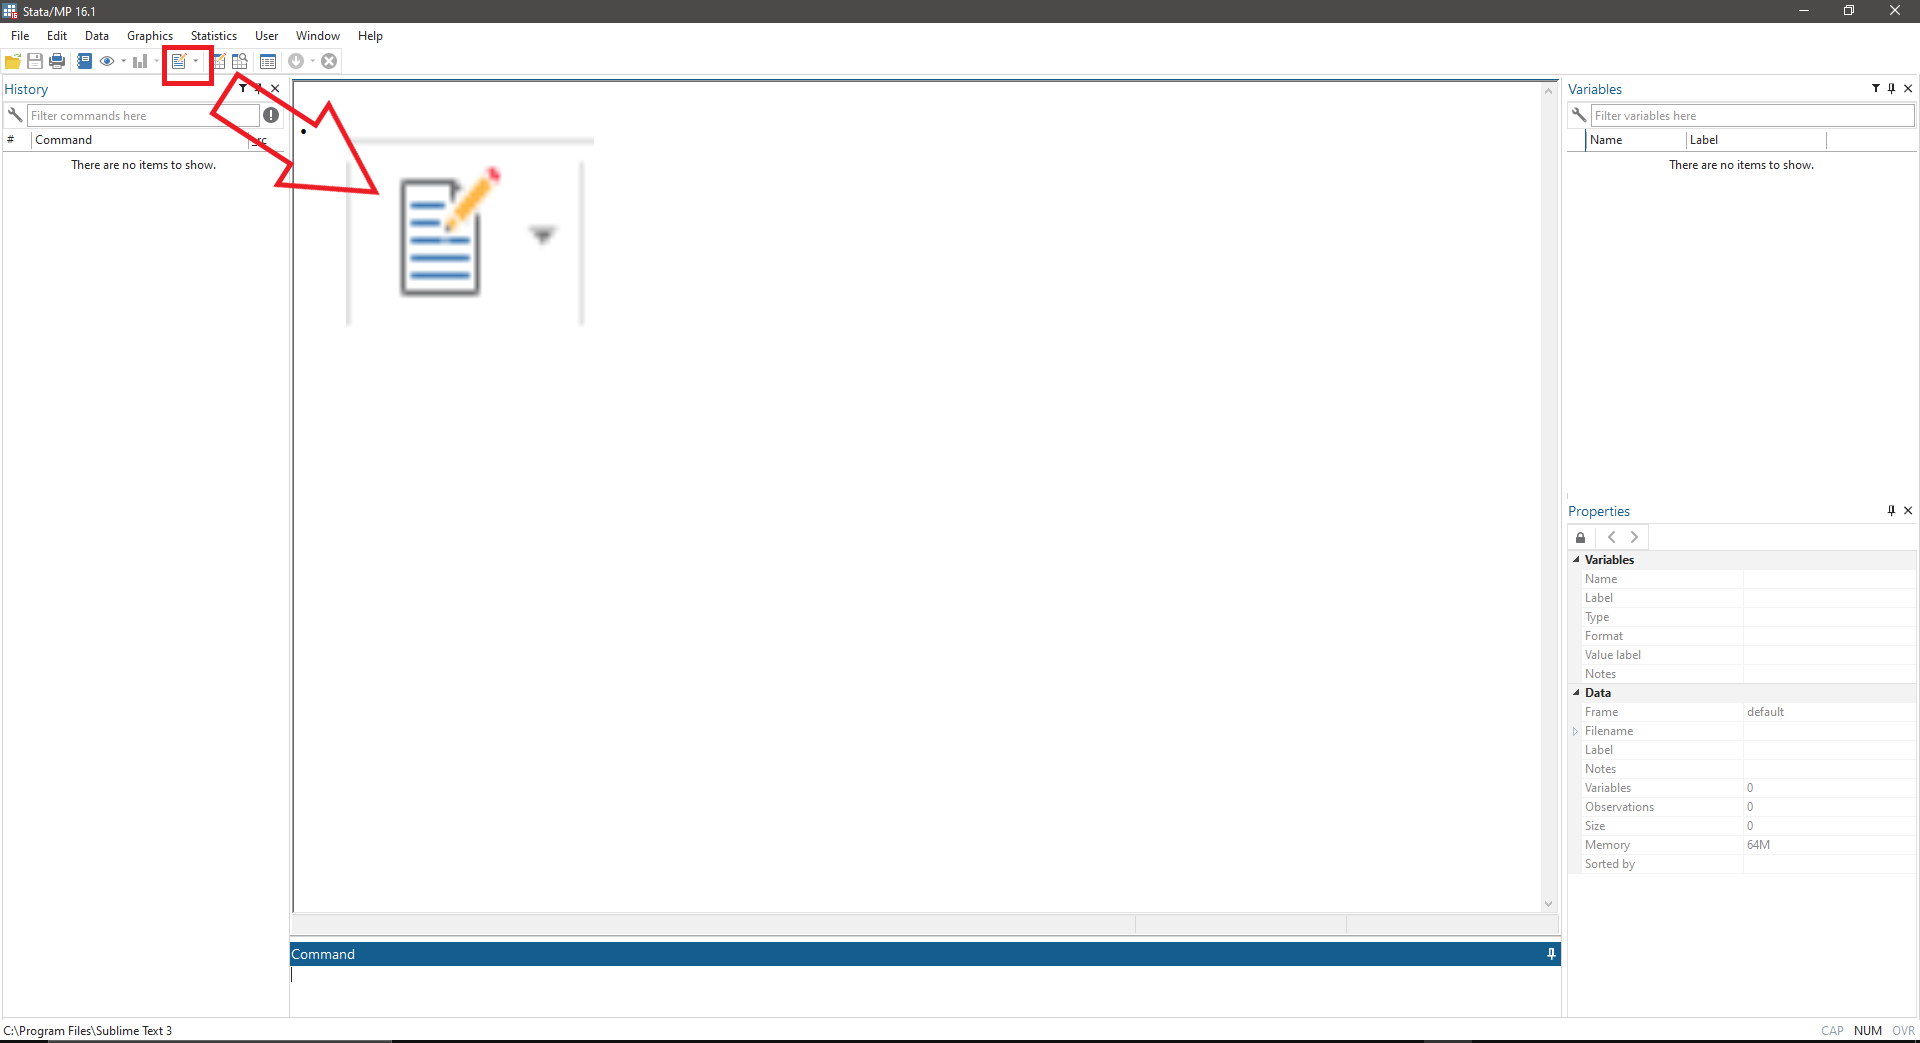
\includegraphics[width = 0.9\linewidth]{fig/Picture8.png}
			\end{figure}
	\end{itemize}
\end{frame}
%---------------------------------------------------
\begin{frame}{El DO-file}
	\begin{itemize}
		\item Puede escribir todos los comandos, procedimientos y c�lculos en este archivo DO; luego, simplemente ejecute el archivo DO y obtendr� secuencialmente todo lo que hiciste.
		\item Puedes enviar por correo electr�nico el archivo DO y mostrar a otros amigos c�mo hiciste, espec�ficamente, algunos c�lculos (�todos los pasos est�n ah�!).
		\item Debes aprender a usar este archivo DO, eso es importante porque necesitas presentar este archivo en la tarea final.
		\item Aqu� una muestra, descargue el archivo DO llamado \textcolor{red}{\href{https://econweb.rutgers.edu/frojas/teaching/undergraduate/do_file_session_monday20.zip}{do file session monday20}}
	\end{itemize}
\end{frame}







